\documentclass[a4paper, 14 pt, titlepage]{extarticle}

\usepackage{grffile}
\usepackage{cmap}					% поиск в PDF
\usepackage[english,russian]{babel}	% локализация и переносы
\usepackage{indentfirst} 
\frenchspacing
\usepackage{setspace}
\usepackage{fontspec}      %% подготавливает загрузку шрифтов Open Type, True Type и др.
\defaultfontfeatures{Ligatures={TeX},Renderer=Basic}  %% свойства шрифтов по умолчанию
\setmainfont[Ligatures={TeX,Historic}]{Times New Roman} 
\setmonofont{Courier New}

\usepackage{amsmath,amsfonts,amssymb} 
\usepackage{amsthm}
\usepackage{mathtools}
\usepackage{icomma}

\renewcommand{\epsilon}{\ensuremath{\varepsilon}}
\renewcommand{\phi}{\ensuremath{\varphi}}
\renewcommand{\kappa}{\ensuremath{\varkappa}}
\renewcommand{\le}{\ensuremath{\leqslant}}
\renewcommand{\leq}{\ensuremath{\leqslant}}
\renewcommand{\ge}{\ensuremath{\geqslant}}
\renewcommand{\geq}{\ensuremath{\geqslant}}
\renewcommand{\emptyset}{\varnothing}

\usepackage{ragged2e}

\usepackage[unicode, pdfencoding=auto]{hyperref}
\usepackage[usenames,dvipsnames,svgnames,table,rgb]{xcolor}
\hypersetup{
            unicode=true,
            colorlinks=true,
            linkcolor=black,
            urlcolor=black,
            citecolor=black
           }

\usepackage{graphicx}
\graphicspath{{images/}}
\usepackage{wrapfig}
\usepackage{tikz}

\usepackage{listings}
\usepackage{color}

\lstset{
	basicstyle=\footnotesize\ttfamily,
	tabsize=4,
	columns=fixed,
	extendedchars=true,
	lineskip=-0.05\baselineskip,
	aboveskip=6pt,
	belowskip=6pt,
	breaklines,
	showstringspaces
}

\usepackage{cite}
\addto\captionsrussian{\renewcommand{\refname}{СПИСОК ИСПОЛЬЗОВАННЫХ ИСТОЧНИКОВ}}
\addto\captionsrussian{\renewcommand{\contentsname}{СОДЕРЖАНИЕ}}
\usepackage[titletoc]{appendix}
\addto\captionsrussian{\renewcommand{\appendixname}{Приложение}}
%\usepackage{tocloft}
%\usepackage{tocstyle}

\usepackage{array,tabularx,tabulary,booktabs, longtable, multirow}

\usepackage{etoolbox}
\usepackage{caption}
\captionsetup{labelsep=endash, font={singlespacing}, figurename=Рисунок }

\usepackage{lastpage}
\usepackage{fancyhdr} % Колонтитулы
 	\pagestyle{fancy}
 	\renewcommand{\headrulewidth}{0pt}  % Толщина линейки сверху
    \fancyfoot[R]{}
    \fancyfoot[C]{\thepage}
    \fancyhead[R]{}
    \fancyhead[L]{}
    
\setstretch{1.5}

\usepackage{extsizes}
\usepackage{geometry}
\geometry{top=2cm}
\geometry{bottom=2cm}
\geometry{left=3cm}
\geometry{right=1.5cm}

\usepackage{titlesec}

\renewcommand{\thesection}{\arabic{section}}
%\titleformat{\section}{\centering\normalsize \normalfont \bfseries }{\thesection}{1ex}{~\\\centering}[]
\titleformat{\section}{\centering\normalsize\normalfont\bfseries\uppercase}{\thesection.}{0.7ex}{}

\renewcommand{\thesubsection}{\thesection.\arabic{subsection}}
\titleformat{\subsection}{\normalsize\normalfont \bfseries}{\thesubsection.}{0.7ex}{}
\titlespacing\subsection{1.25cm}{1cm}{0pt}

\renewcommand{\thesubsubsection}{\thesubsection.\arabic{subsubsection}}
\titleformat{\subsubsection}{\normalsize\normalfont}{\thesubsubsection.}{0.7ex}{}
\titlespacing\subsubsection{1.25cm}{1cm}{0pt}

%\parindent=1.25cm
\setlength{\parindent}{1.25cm}

\newcommand{\startcode}{
    \footnotesize
    \singlespacing
}

\newcommand{\finishcode}{\setstretch{1.5}\normalsize}

\newenvironment{code}{\startcode}{\finishcode}

\newcommand{\printcaption}[1]{
    \normalsize
    {
    \captionsetup{justification=raggedright, singlelinecheck=off}
    \caption{#1}
    }
}




\newcommand{\teacher}{Преподавателев~П.П.}
\newcommand{\theme}{Наименование темы}
\newcommand{\firstmember}{Иванов~И.И.}
\newcommand{\secondmember}{Петров~П.П.}
\newcommand{\thirdmember}{Сидоров~С.С.}
\newcommand{\groupnumber}{0000}
\newcommand{\group}{Группа 0000}

\begin{document}

\begin{titlepage}
   
   \begin{center}
       {\linespread{1.5}
        \textbf{
             МИНОБРНАУКИ РОССИИ\\
             САНКТ-ПЕТЕРБУРГСКИЙ
             ГОСУДАРСТВЕННЫЙ
             ЭЛЕКТРОТЕХНИЧЕСКИЙ
             УНИВЕРСИТЕТ\\ <<ЛЭТИ>> ИМ.~
             В.И.~УЛЬЯНОВА (ЛЕНИНА)\\
            Кафедра МО ЭВМ\\
            \vspace{7cm}
            ОТЧЁТ\\
            по учебной практике\\
            Тема: \theme\\
        }
        
        \vspace{4cm}
        
       
       
       \setlength{\extrarowheight}{4mm}
       \begin{tabulary}{\textwidth}{LCCCL}
            Студент гр. \groupnumber & \hspace{0.5cm} & \hspace{4.5cm} & \hspace{0.5cm} & \firstmember \\
            \cline{3-3}
            Студент гр. \groupnumber & \hspace{0.5cm} & \hspace{4.5cm} & \hspace{0.5cm} & \secondmember \\
            \cline{3-3}
            Студент гр. \groupnumber & \hspace{0.5cm} & \hspace{4.5cm} & \hspace{0.5cm} & \thirdmember \\
            \cline{3-3}
            Руководитель & \hspace{0.5cm} & \hspace{4.5cm} & \hspace{0.5cm} & \teacher \\
            \cline{3-3}
       \end{tabulary}
       \setlength{\extrarowheight}{0mm}
       
       \vfill
       
       Санкт-Петербург\\
       \the\year\\
       }
       
   \end{center}
   
  \end{titlepage}




\setcounter{page}{2}

\section*{Задание\\ на учебную практику}

\setlength{\extrarowheight}{7mm}
\begin{tabularx}{\textwidth}{>{\raggedright\arraybackslash}X}
	Студент \firstmember{} группы \groupnumber\\
	Студент \secondmember{} группы \groupnumber\\
	Студент \thirdmember{} группы \groupnumber\\
	Тема практики: \theme \\
	Задание на практику: Командная итеративная разработка визуализатора алгоритма на Java с графическим интерфейсом. Алгоритм: \ldots\\
	Сроки прохождения практики: 00.00.0000 -- 00.00.0000\\
	Дата сдачи отчёта: 00.00.0000\\
	Дата защиты отчёта: 00.00.0000\\
\end{tabularx}
\setlength{\extrarowheight}{0mm}

\vspace{50mm}
%\vfill

\setlength{\extrarowheight}{4mm}
       \begin{tabulary}{\textwidth}{LCCCL}
            Студент & \hspace{0.5cm} & \hspace{4.5cm} & \hspace{0.5cm} & \firstmember \\
            \cline{3-3}
            Студент & \hspace{0.5cm} & \hspace{4.5cm} & \hspace{0.5cm} & \secondmember \\
            \cline{3-3}
            Студент & \hspace{0.5cm} & \hspace{4.5cm} & \hspace{0.5cm} & \thirdmember \\
            \cline{3-3}
            Руководитель & \hspace{0.5cm} & \hspace{4.5cm} & \hspace{0.5cm} & \teacher \\
            \cline{3-3}
       \end{tabulary}
       \setlength{\extrarowheight}{0mm}

\newpage

\section*{АННОТАЦИЯ}
\begin{minipage}[t][0.4\textheight][t]{0.9\linewidth}
	\setlength{\parindent}{1.25cm}
	\indent
	Задачей учебной практики является \ldots\ Практика заключается в \ldots\ Разработка ведётся \ldots\
	
	В отчёте приведена информация о \ldots\
\end{minipage}

\selectlanguage{english}
\section*{SUMMARY}
\begin{minipage}[t][0.4\textheight][t]{0.9\linewidth}
	\setlength{\parindent}{1.25cm}
	\indent
	Summary in English.
\end{minipage}
\selectlanguage{russian}

\newpage

\let \savenumberline \numberline
\def \numberline#1{\savenumberline{#1.}}

\tableofcontents

\newpage

\section*{Введение}
\addcontentsline{toc}{section}{Введение}

Целью работы является \ldots\ Для достижения цели необходимо решить следующие задачи:

\begin{enumerate}
	\item \ldots;
	\item \ldots;
\end{enumerate}

В данной работе визуализируется алгоритм \ldots

\newpage

\section{Требования к программе}

\subsection{Исходные требования к программе.}

\subsubsection{Требования ко входным данным.}

Текст.

\subsubsection{Требования к визуализации процесса выполнения алгоритма.}

Текст.

\subsubsection{Требования к пользовательскому интерфейсу.}

Текст.

\subsection{Уточнения требований после сдачи прототипа.}

\begin{enumerate}
	\item
	\item 
	\item 
\end{enumerate}

\subsection{Уточнения требований после сдачи первой версии.}

\begin{enumerate}
	\item 
	\item 
	\item 
\end{enumerate}

\subsection{Уточнения требований после сдачи второй версии.}
\begin{enumerate}
	\item 
	\item 
	\item 
\end{enumerate}

\newpage
\section{План разработки и распределение ролей в бригаде}

\subsection{План разработки.}

\begin{enumerate}
	\item К 0 июля — $\ldots$
	\item К 0 июля — $\ldots$
	\item К 0 июля — $\ldots$
	\item К 0 июля — $\ldots$
\end{enumerate}

\subsection{Распределение ролей в бригаде.}

\begin{itemize}
	\item \firstmember{} — разработка \ldots
	\item \secondmember{} — разработка \ldots
	\item \thirdmember{} — разработка \ldots
\end{itemize}

\newpage
\section{Особенности реализации}
\subsection{Структуры данных.}

\subsection{Основные методы.}

\newpage
\section{Тестирование}

\subsection{Тестирование графического интерфейса.}

\begin{figure}[h!]
	\centering
	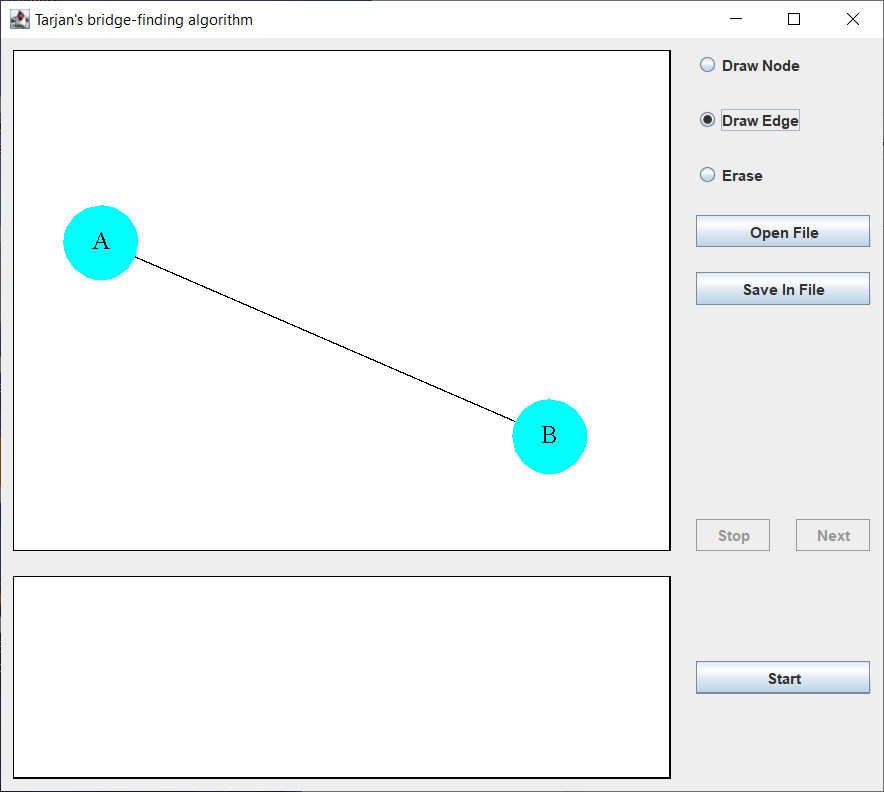
\includegraphics[width=0.8\linewidth]{screenshots/1}
	\caption{Наименование иллюстрации}
	\label{fig:my-unique-label}
\end{figure}

\subsection{Тестирование кода алгоритма.}

\newpage
\section*{Заключение}
\addcontentsline{toc}{section}{Заключение}
Кратко подвести итоги, проанализировать соответствие поставленной цели и полученного результата.

\newpage

\addcontentsline{toc}{section}{Список использованных источников}
\begin{thebibliography}{99}
	\bibitem{} Иванов И. И. Книга одного-трех авторов. М.: Издательство, 2010. 000 с.
	\bibitem{} Книга четырех авторов / И. И. Иванов, П. П. Петров, С. С. Сидоров, В. В. Васильев. СПб.: Издательство, 2010. 000 с.
	\bibitem{} Книга пяти и более авторов / И. И. Иванов, П. П. Петров, С. С. Сидоров и др.. СПб.: Издательство, 2010. 000 с.
	\bibitem{} Описание книги под редакцией / под ред. И.И. Иванова СПб., Издательство, 2010. 000 с.
	\bibitem{} Иванов И.И. Описание учебного пособия и текста лекций: учеб. пособие. СПб.: Изд-во СПбГЭТУ «ЛЭТИ», 2010. 000 с.
	\bibitem{} Описание методических указаний / сост.: И.И. Иванов, П.П. Петров. СПб.: Изд-во СПбГЭТУ «ЛЭТИ», 2010. 000 с.
	\bibitem{} Иванов И.И. Описание статьи с одним-тремя авторами из журнала // Название журнала. 2010, вып. (№) 00. С. 000–000.
	\bibitem{} Описание статьи с четырьмя и более авторами из журнала / И. И. Иванов, П. П. Петров, С. С. Сидоров и др. // Название журнала. 2010, вып. (№) 00. С. 000–000.
	\bibitem{} Иванов И.И. Описание тезисов доклада с одним-тремя авторами / Название конференции: тез. докл. III международной науч.-техн. конф., СПб,  00–00 янв. 2000 г. / СПбГЭТУ «ЛЭТИ», СПБ, 2010, С. 000–000.
	\bibitem{} Описание тезисов доклада с четырьмя и более авторами / И. И. Иванов, П. П. Петров, С. С. Сидоров и др. // Название конференции: тез. докл. III международной науч.-техн. конф., СПб,  00–00 янв. 2000 г. / СПбГЭТУ «ЛЭТИ», СПБ, 2010, С. 000–000.
	\bibitem{} Описание электронного ресурса // Наименование сайта. URL: http://east-front.narod.ru/memo/latchford.htm (дата обращения: 00.00.2010).
	\bibitem{} ГОСТ 0.0–00. Описание стандартов. М.: Изд-во стандартов, 2010.
	\bibitem{} Пат. RU 00000000. Описание патентных документов / И. И. Иванов, П. П. Петров, С. С. Сидоров. Опубл. 00.00.2010. Бюл. № 00.
	\bibitem{} Иванов И.И. Описание авторефератов диссертаций: автореф. дисс. канд. техн. наук / СПбГЭТУ «ЛЭТИ», СПБ, 2010.
	\bibitem{} Описание федерального закона: Федер. закон [принят Гос. Думой 00.00.2010] // Собрание законодательств РФ. 2010. № 00. Ст. 00. С. 000–000.
	\bibitem{} Описание федерального постановления: постановление Правительства Рос. Федерации от 00.00.2010 № 00000 // Опубликовавшее издание. 2010. № 0. С. 000–000.
	\bibitem{} Описание указа: указ Президента РФ от 00.00.2010 № 00 // Опубликовавшее издание. 2010. № 0. С. 000–000.
\end{thebibliography}

\newcommand{\sectionset}{\centering\normalsize\normalfont\bfseries\expandafter\uppercase}
\titleformat{\section}{\centering\normalsize\normalfont\bfseries}{}{0ex}{ПРИЛОЖЕНИЕ \thesection\\\uppercase}{}
\begin{appendices}
\renewcommand{\thesection}{\Asbuk{section}}

\newpage
\section{UML-диаграмма классов}\label{appendix:UML}

UML-диаграмма классов проекта представлена на рисунке ниже.

\newpage
\section{Исходный код программы}\label{appendix:code}
Название файла: \ldots

\begin{lstlisting}
	class HelloWorld {
		public static void main(String[] args) {
			System.out.println("Hello, World!"); 
		}
	}
\end{lstlisting}

\newpage
\section{Результаты тестирования программы}\label{appendix:test}


\end{appendices}
\end{document}